\documentclass{article}
\usepackage{graphicx} % Required for inserting images
\usepackage{indentfirst}
\graphicspath{ {./images/} }
\usepackage{url}

\title{Physics of Cosmic Rays - Final Design Brief}
\author{Dylan Krulewitz, Hugh Jones, Addison Cate }
\date{April 2025}

\begin{document}

\maketitle

\section{Introduction}

The average person is completely oblivious to the cosmic particles flying through them at all times. The focus of this course is to reveal the unseen in a dynamic way. While many may feel like physics is not for them, this project explores how design can make complex scientific topics accessible, and ignite the innate human curiosity within. Our group was given the topic of planes, so we explored how two-dimensional surfaces could create points of reference for the cosmic rays to pass through. This way, the planes could be compared to the scintillator or various layers of the atmosphere. 

As a group, we learned to stay open to various design discoveries, and routinely experiment with new ideas. Some of the highlights of our project were originally unplanned, showing how remaining fluid in the process opens up your mind to new possibilities. By exploring the interaction between elements, like materials and light for example, we can create new layers of intrigue and complexity, which can spark the curiosity of viewers. 


\section{Thesis Statement}
Our 12” x 12” prototype explores how design principles can express the physics of cosmic rays through the interactions of patterned light with planar surfaces.

\section{Investigative Process}
Throughout the project, our groups employed an iterative process integrated with thoughtful precedent research and reflection. 

We began our research with a reading on epistemology, delving into how humans establish truth. This exercise in curiosity and exploring the boundaries of knowledge set the tone for the course. Next, our team investigated interactive installation precedent studies, exploring the interplay between the senses, user input, and technology. This created a foundation in installation design for our future experimentation. As a collective, we then drew upon the lessons of the reading in order to distill what questions were most valuable to pursue. As a whole, we realized that inspiring awe and cultivating curiosity were the common goals. Next, our group explored early prototyping abstract models inspired by the touch of code chapter on exploration. 
\begin{figure} [h]
    \centering
  \begin{minipage}[b]{0.4\textwidth}
    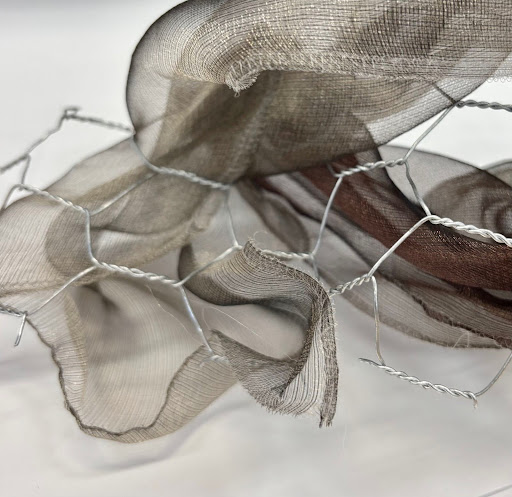
\includegraphics[width=\textwidth]{images/unnamed.jpg}
  \end{minipage}
  \hfill
  \begin{minipage}[b]{0.4\textwidth}
    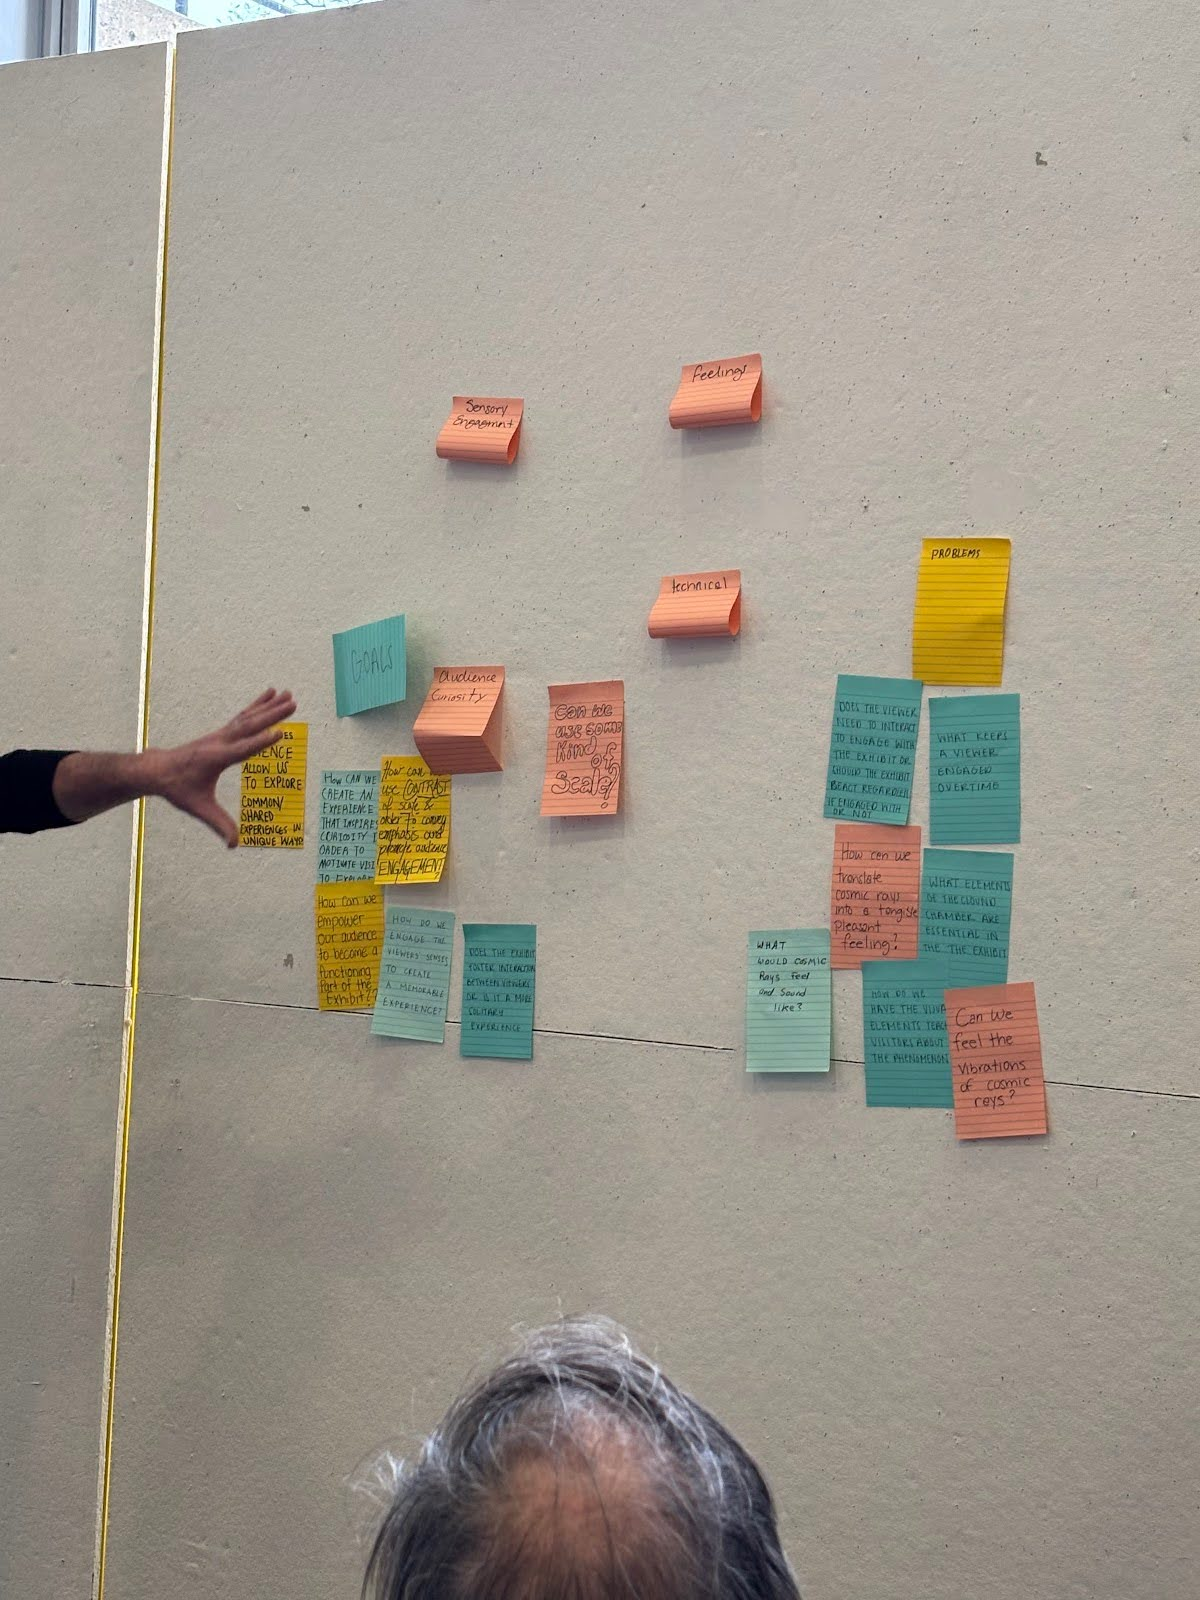
\includegraphics[width=\textwidth]{images/unnamed2.jpg}
  \end{minipage}
\end{figure}

We then transitioned to the primary project of the course, the 12” x 12” model examining planar surfaces. We began with a system of suspended planes with LEDs shooting through, however, our team received feedback that flat planes were too linear, and the box needed more user interaction. With that critique in mind, our initial box was a throwaway cardboard concept, featuring cut up CDs and rubberbands. Although it wasn’t very polished, the first prototype was the crucial first experimentation in light interaction, reflective surfaces, and user interaction.

\begin{figure} [h]
    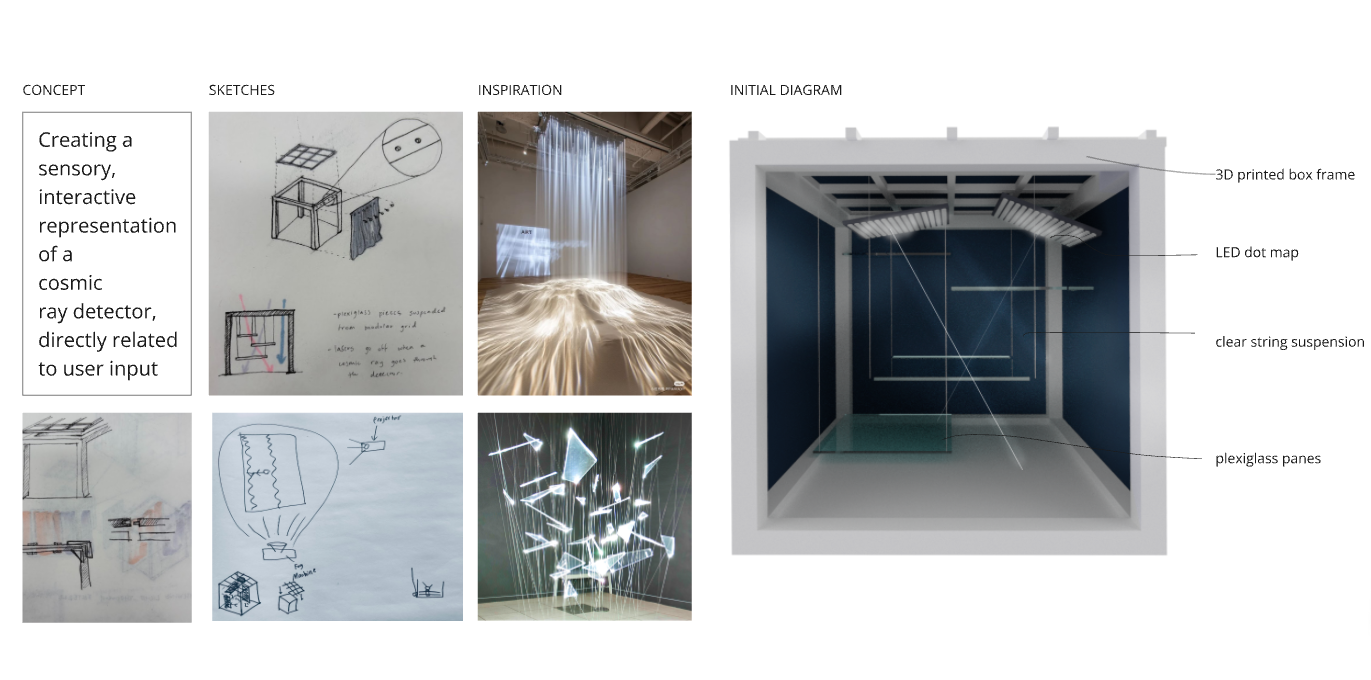
\includegraphics[width=1\linewidth]{images/unnamed3.png}
\end{figure}

\begin{figure} [h]
    \centering
  \begin{minipage}[b]{0.4\textwidth}
    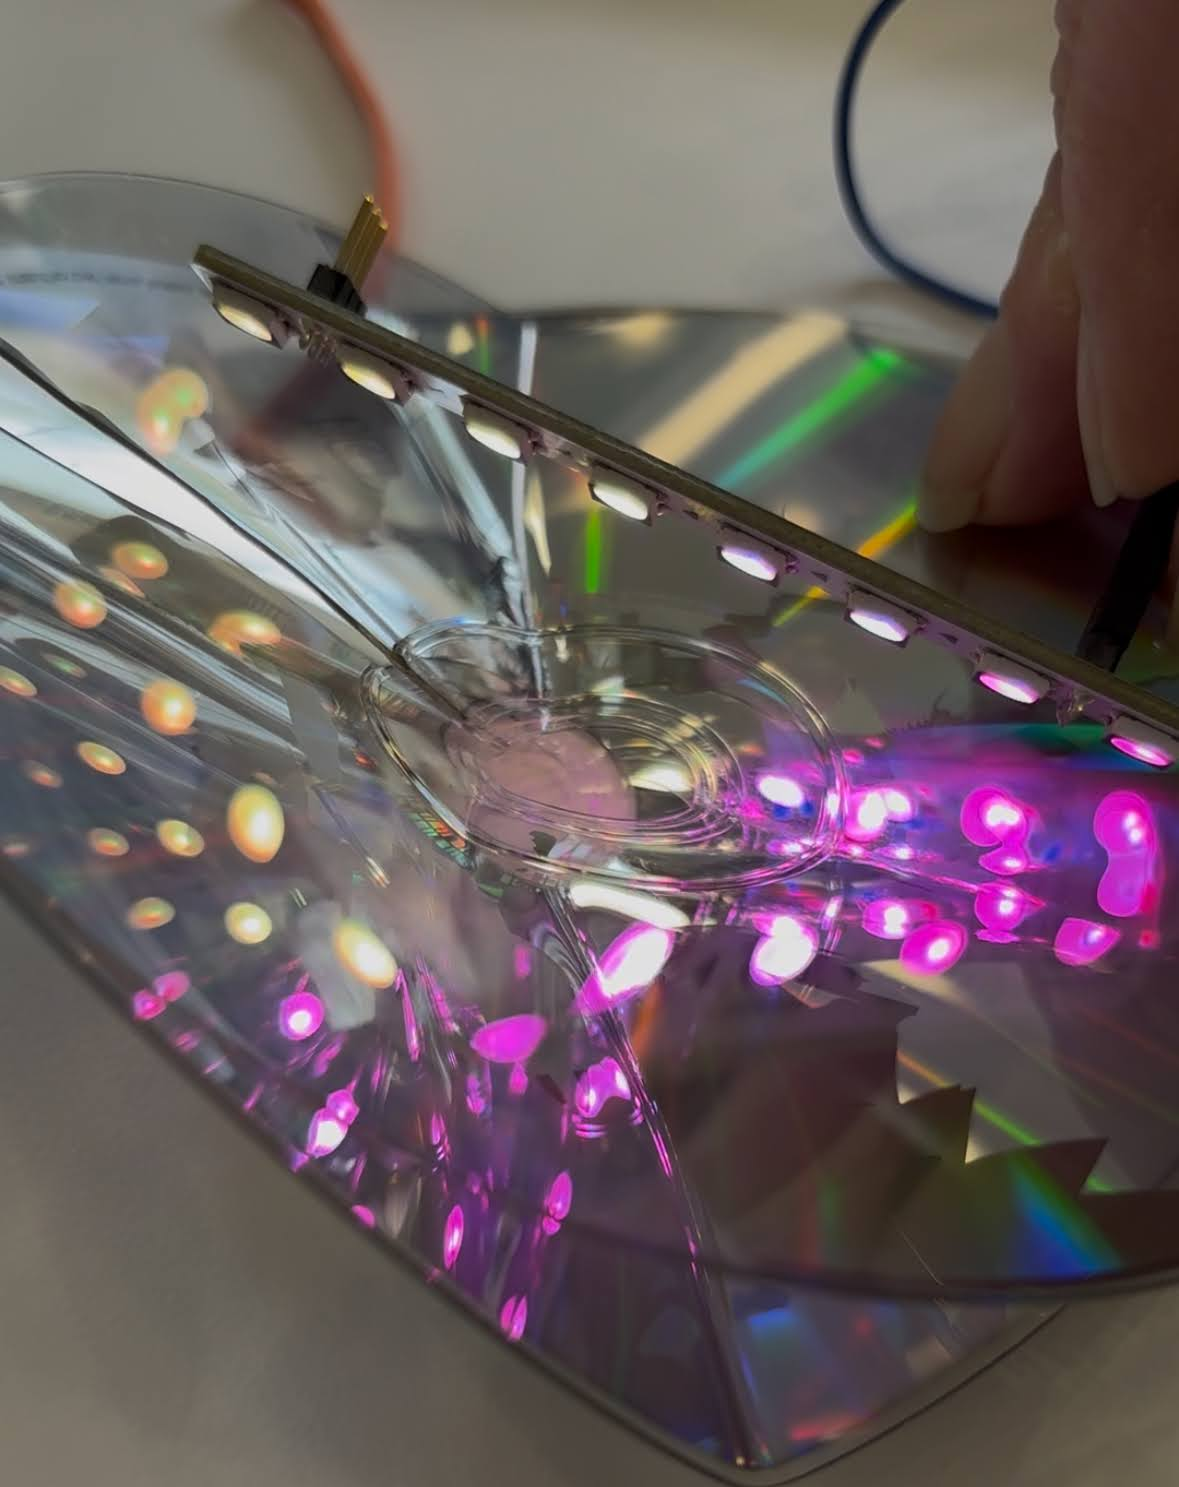
\includegraphics[width=\textwidth]{images/unnamed4.jpg}
  \end{minipage}
  \hfill
  \begin{minipage}[b]{0.4\textwidth}
    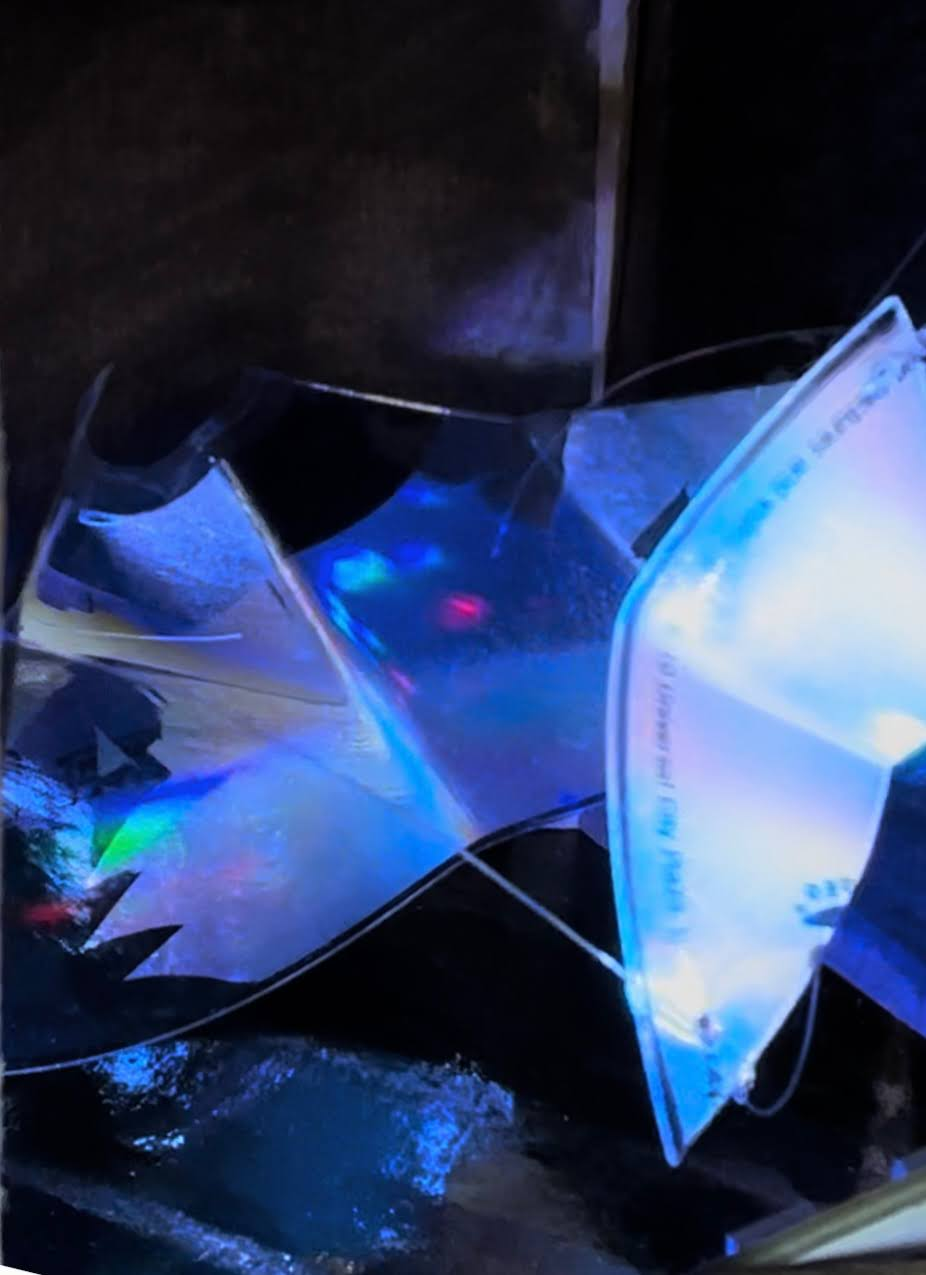
\includegraphics[width=\textwidth]{images/unnamed5.jpg}
  \end{minipage}
\end{figure}

With our next box iteration, we intended to focus on scattering light through planar surfaces. Magnets would also provide the increased interaction desired from mid-review. The increased layering from light reflections would reference the increasing complexity that results from cosmic showers. In addition, as we moved towards a more developed box design, joints were tested in order to create a box that would provide the most flexibility and modularity. 

\begin{figure} [h]
    \centering
    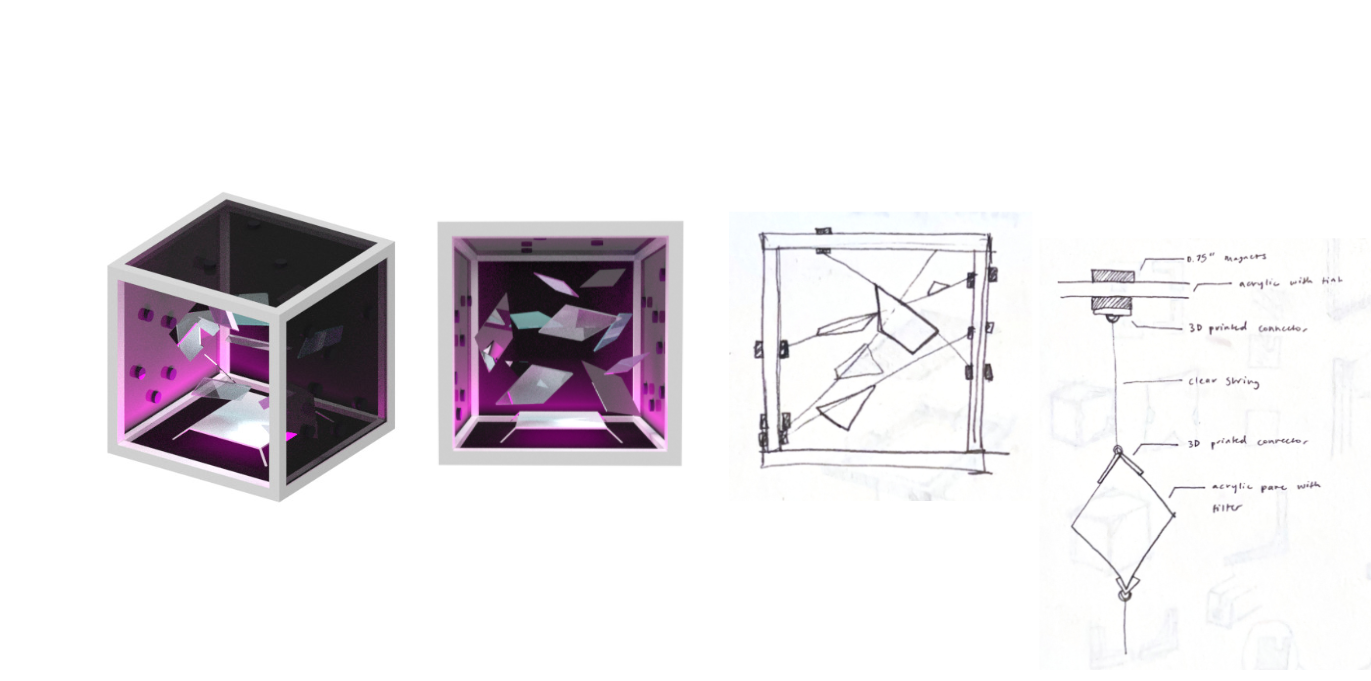
\includegraphics[width=1\linewidth]{images/unnamed6.png}
\end{figure}

Next, readings on Robert Irwin and Edward Tufte broadened our perspectives and provided theories of psychology and design for us to integrate into our project. Irwin’s reading, for instance, explored the intersection between art and science, highlighting how both disciplines can push the boundaries of perception and knowing. Tufte’s reading was valuable in the design of our diagrams and poster, focusing on clear visual communication, and layered information design. During this phase, we also revisited the cloud chamber, getting back to the source of our scientific inquiry. We utilized this renewed inspiration to drive our further box development. 

\begin{figure} [h]
    \centering
  \begin{minipage}[b]{0.25\textwidth}
    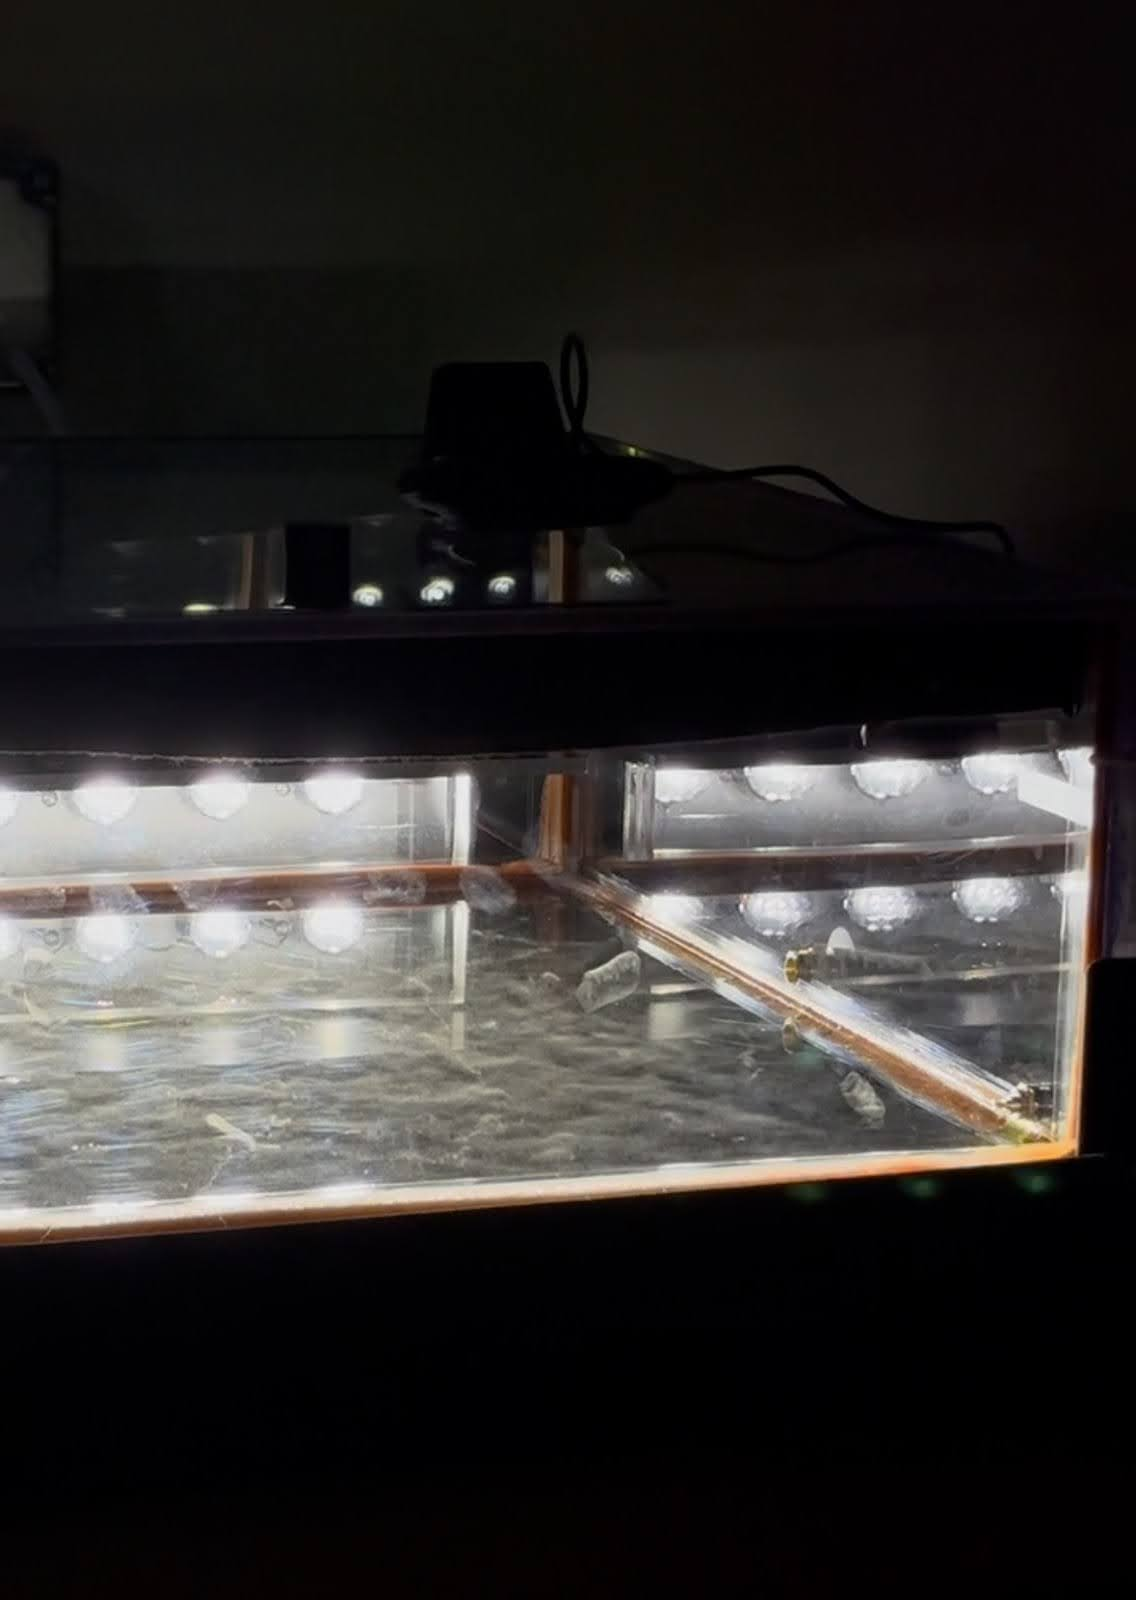
\includegraphics[width=\textwidth]{images/unnamed7.jpg}
  \end{minipage}
  \hfill
  \begin{minipage}[b]{0.25\textwidth}
    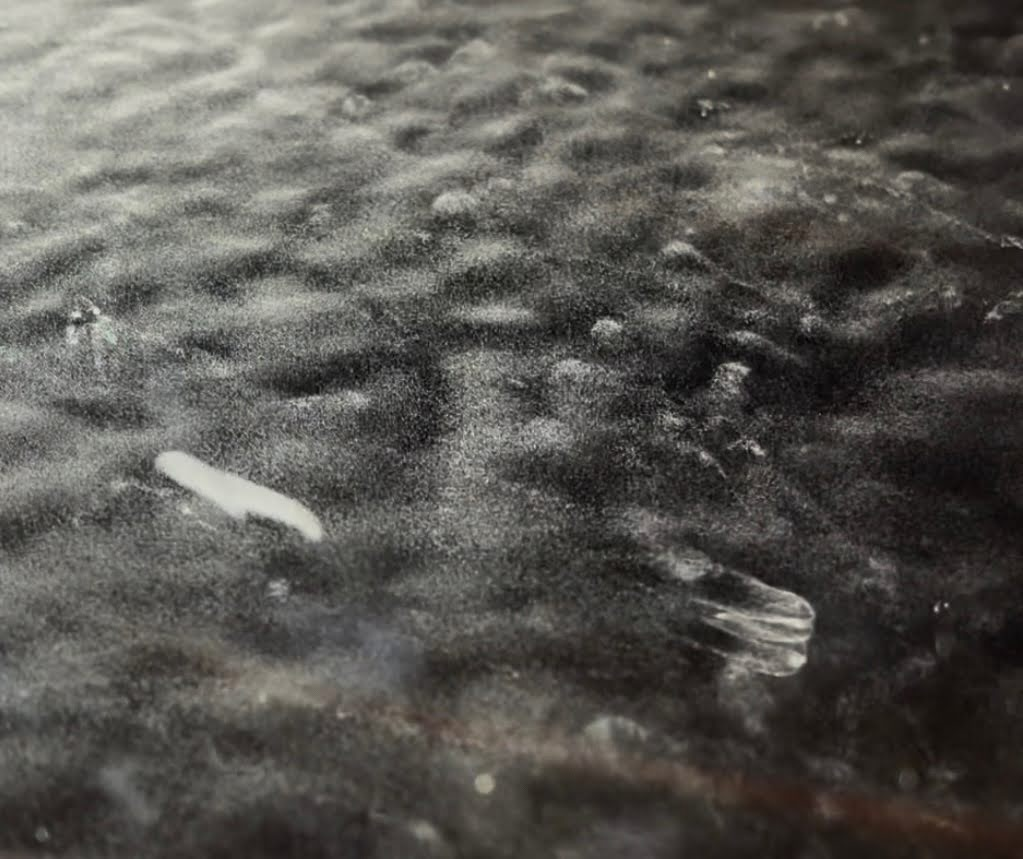
\includegraphics[width=\textwidth]{images/unnamed8.jpg}
  \end{minipage}
  \hfill
  \begin{minipage}[b]{0.25\textwidth}
    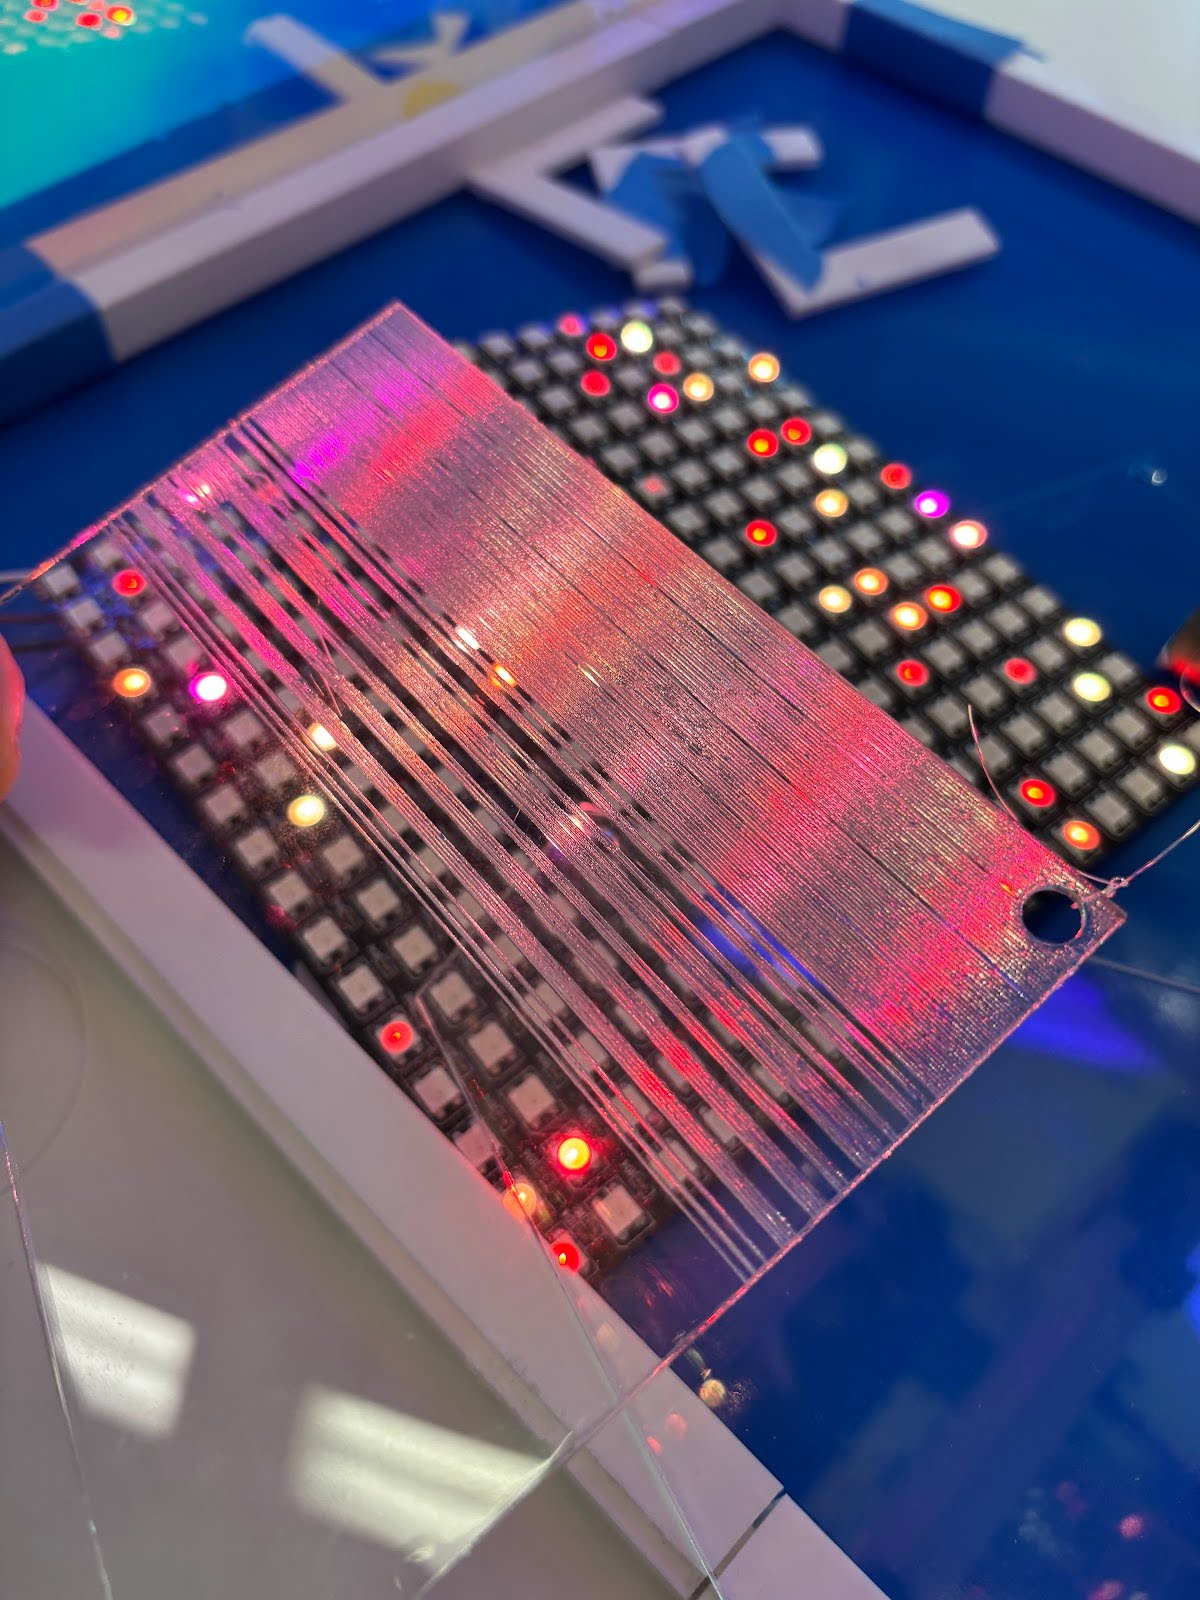
\includegraphics[width=\textwidth]{images/unnamed9.jpg}
  \end{minipage}
\end{figure}

In preparation for Eureca, research into physics concepts was synthesized into simple graphic diagrams, distilling only the key information.

\begin{figure} [h]
    \centering
  \begin{minipage}[b]{0.4\textwidth}
    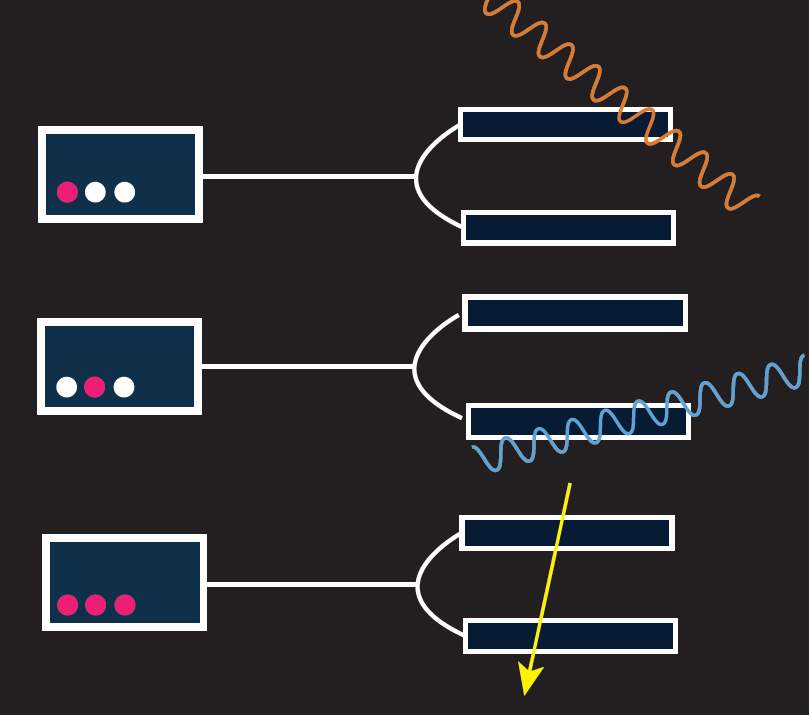
\includegraphics[width=\textwidth]{images/unnamed10.png}
  \end{minipage}
  \hfill
  \begin{minipage}[b]{1\textwidth}
    
\includegraphics[width=\textwidth]{images/unnamed11.png}
  \end{minipage}
\end{figure}

\newpage

Later, further iterations on the LED matrix and strips were introduced. The matrix had an unexpected interaction with the dichroic film, creating a fascinating display of color and reflection. The mirrored film reflected certain colors back, with less variety each time. In a way, this process could be compared to how the particles in a cosmic ray shower eventually decay to muons by the time they reach Earth. 

\begin{figure}[h]
    \centering
  \begin{minipage}[b]{0.35\textwidth}
    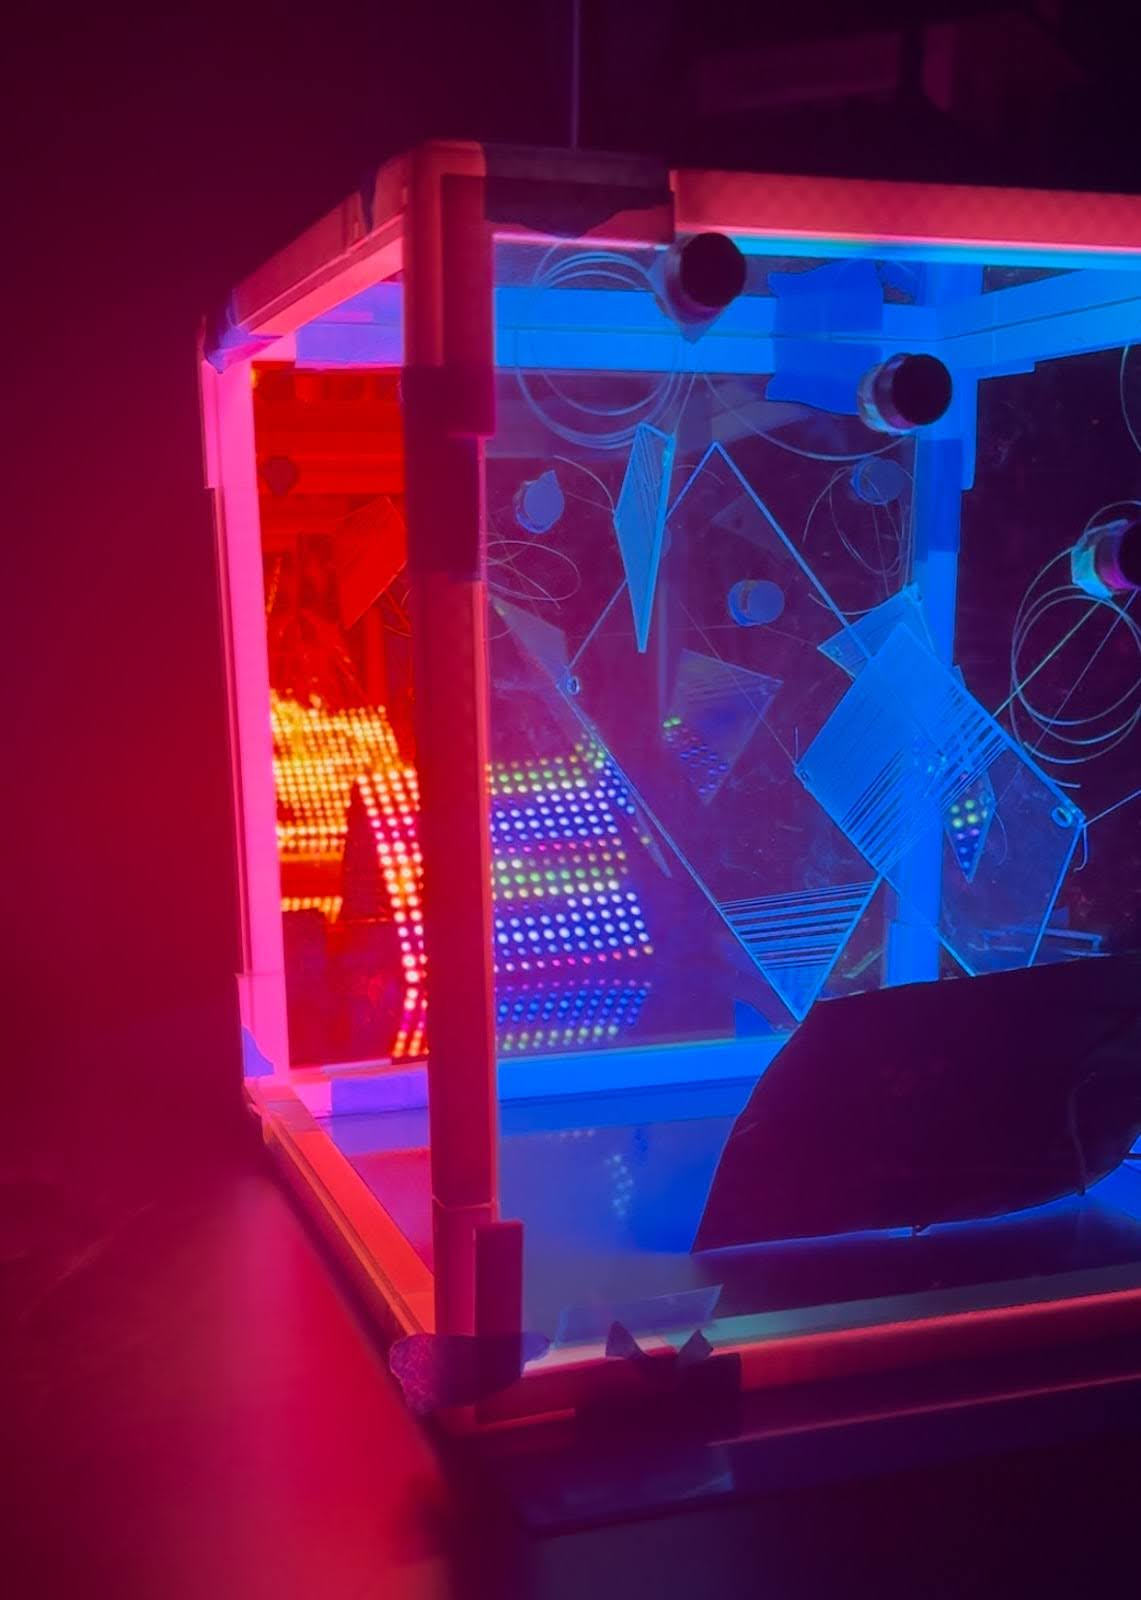
\includegraphics[width=\textwidth]{images/unnamed12.jpg}
  \end{minipage}
  \hfill
  \begin{minipage}[b]{0.35\textwidth}
    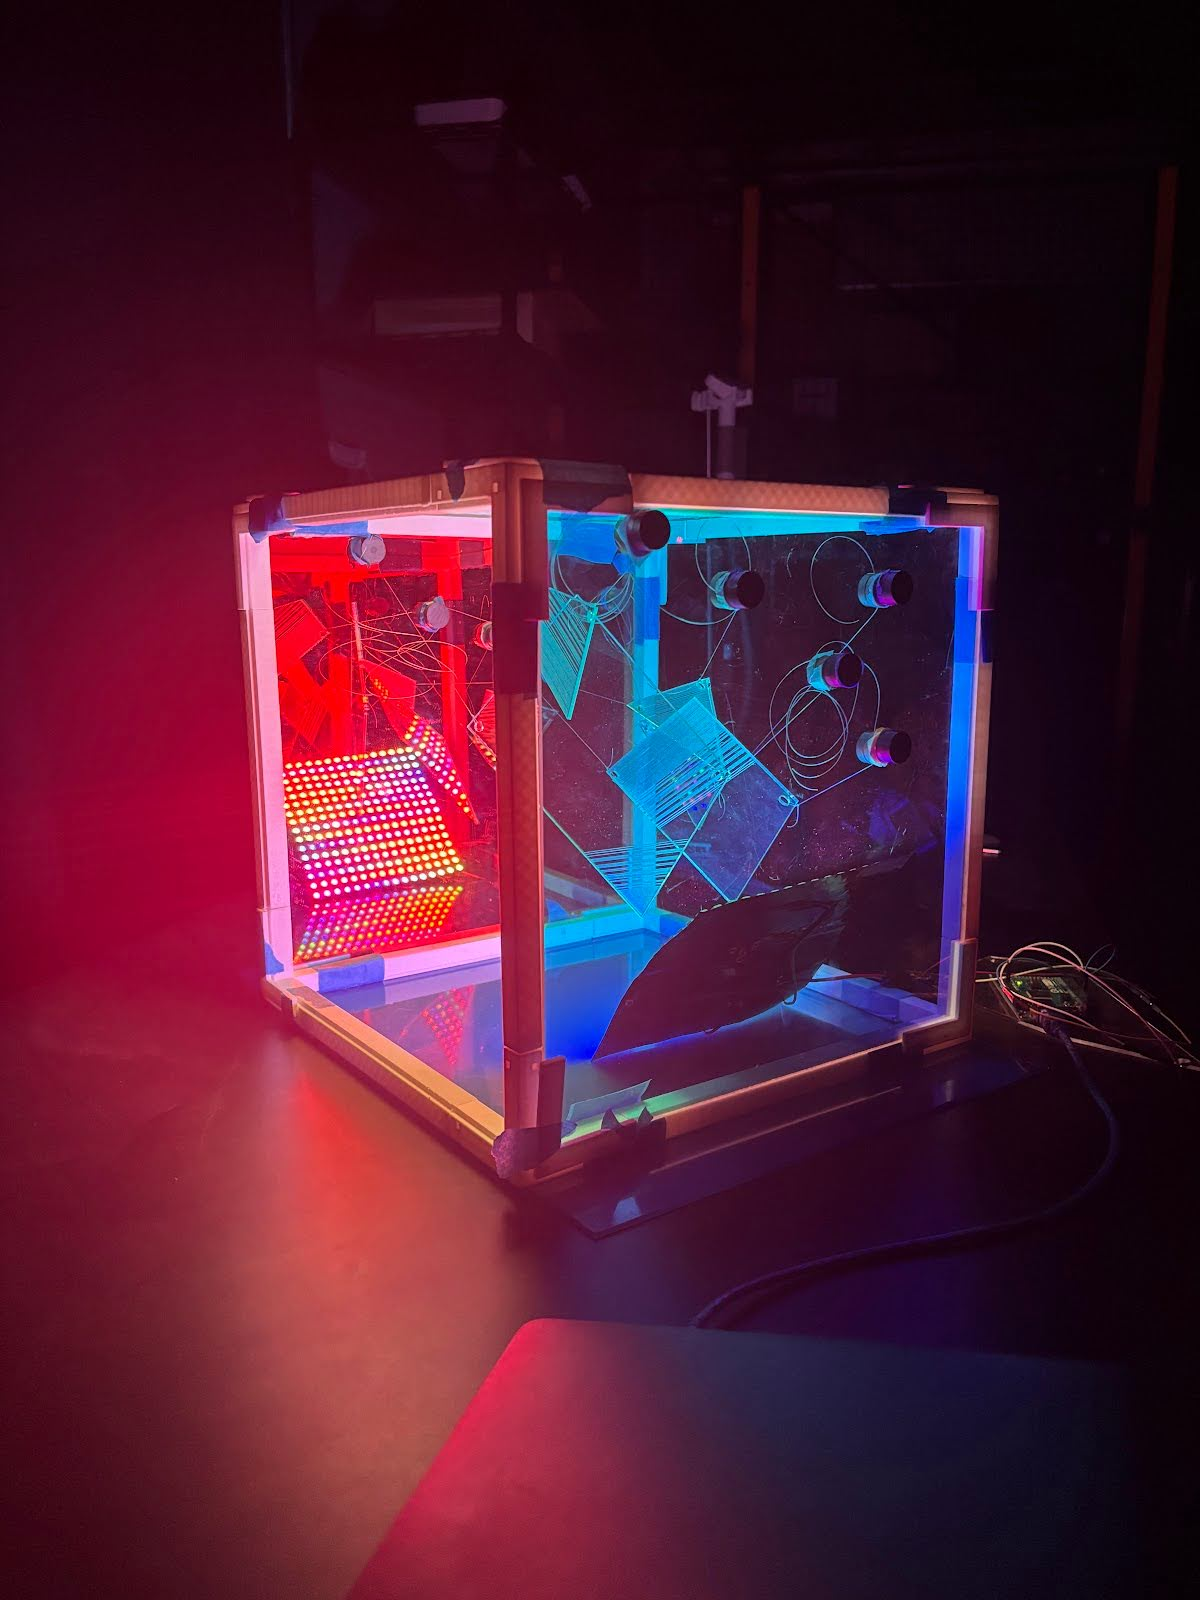
\includegraphics[width=\textwidth]{images/unnamed13.jpg}
  \end{minipage}
\end{figure}

Our final design included the addition of LED strips, referencing cosmics traveling through space. The code was altered in order to create a more dynamic particle path. Through multiple iterations, the two displays were able to strive towards synthesis, rather than two separate phenomena. We also received feedback to further investigate layers of frosted acrylic to reference the atmosphere, so that could be an avenue for future experimentation. 

\begin{figure}[h]
    \centering
  \begin{minipage}[b]{0.35\textwidth}
    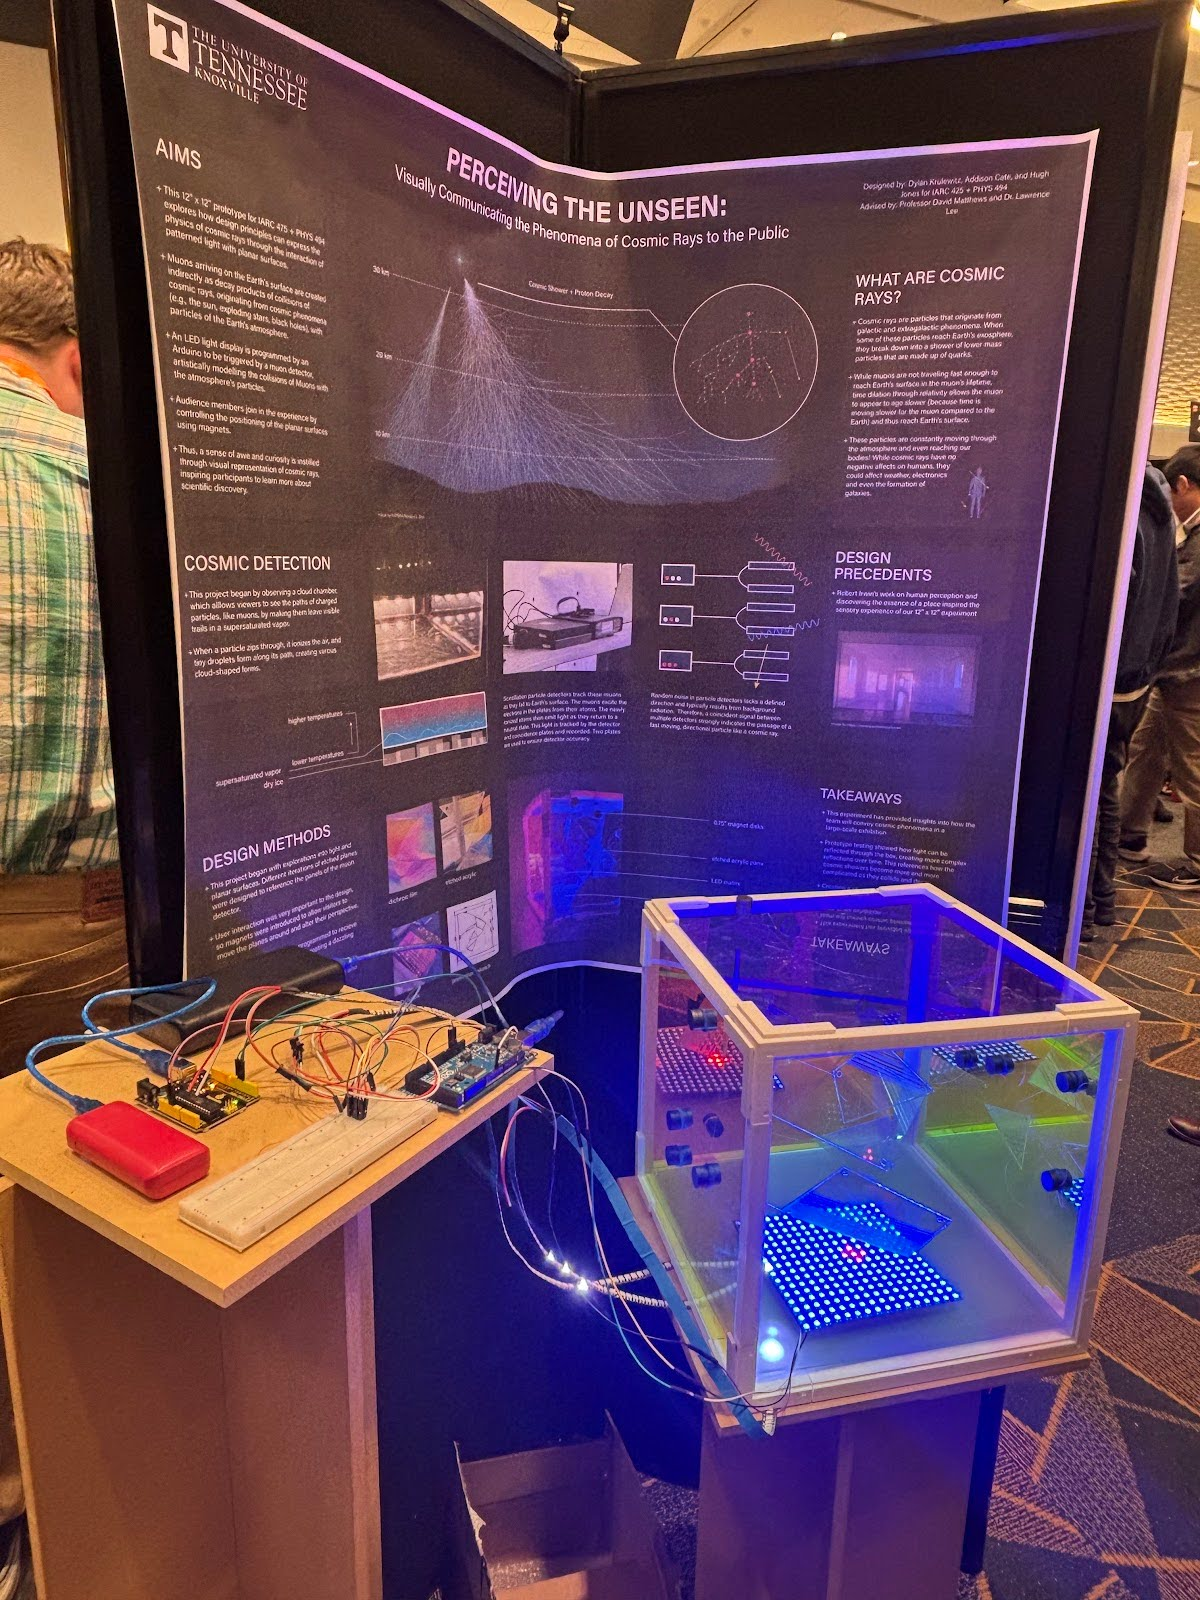
\includegraphics[width=\textwidth]{images/unnamed14.jpg}
  \end{minipage}
  \hfill
  \begin{minipage}[b]{0.35\textwidth}
    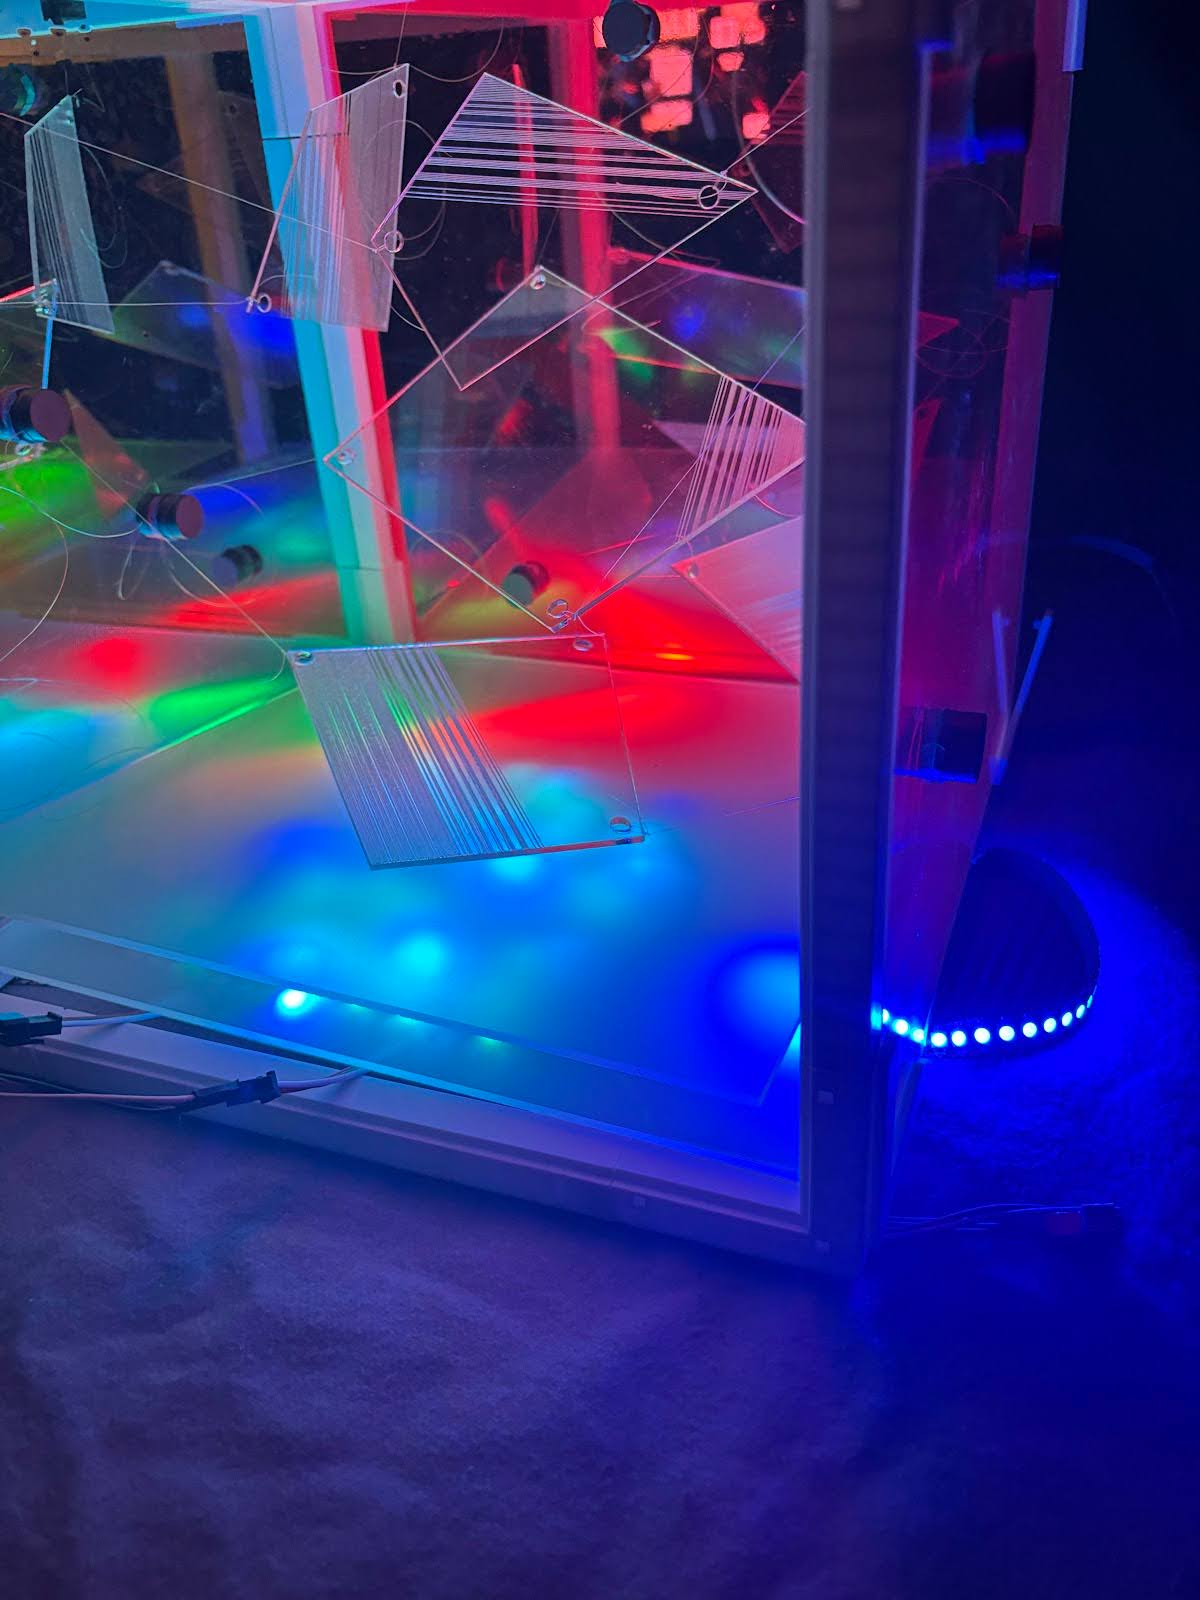
\includegraphics[width=\textwidth]{images/unnamed15.jpg}
  \end{minipage}
\end{figure}

\newpage

\section{Outcomes}
The background gained on abstract design influenced the suspended plexiglass panes within the prototype. One of the reasons we included this part of our design was that we had to implement ideas of two-dimensional geometry into the prototype. The suspended plexiglass panes are etched to allow light to be diffracted throughout the design. The sequence of light diffracting and reflecting throughout the prototype mimics the chaos of the cosmic rays in our upper atmosphere. We implemented two programs in the final prototype for our two LED displays. Both programs used an Arduino Board, the application Arduino IDE, and the programming language C++. We also used the FastLed library as a baseline for our programs. The animation on the LED matrix depicts the event of protons from cosmic phenomena colliding with atoms in our atmosphere to begin a cascade of particle showers. The display on the LED strips represents the various protons moving through the upper atmosphere as cosmic showers are produced. The showers are made up of particles colliding with more atoms, each other, and decaying into more products. Some of these products are particles called muons (which can be described as a more massive electron). A scintillator particle detector receives muons as they fall through our atmosphere. When it detects a muon, it sends a positive signal. We didn’t get the opportunity to use a particle detector during the semester, but the code for the LED strips is prepared to receive a signal from a detector to trigger the LED animation. The lively and colorful displays instilled a sense of awe into our guest viewers. This in turn, gave the audience the inspiration and motivation to learn more about cosmic rays. Our prototype received compliments toward the inclusion of some form of showcasing the cosmic shower. However, the pieces of plexiglass received criticism on their implementation. Reviewers suggested modifications toward enhancing their purpose in the overall design.

\begin{figure}[h]
    \centering
  \begin{minipage}[b]{0.4\textwidth}
    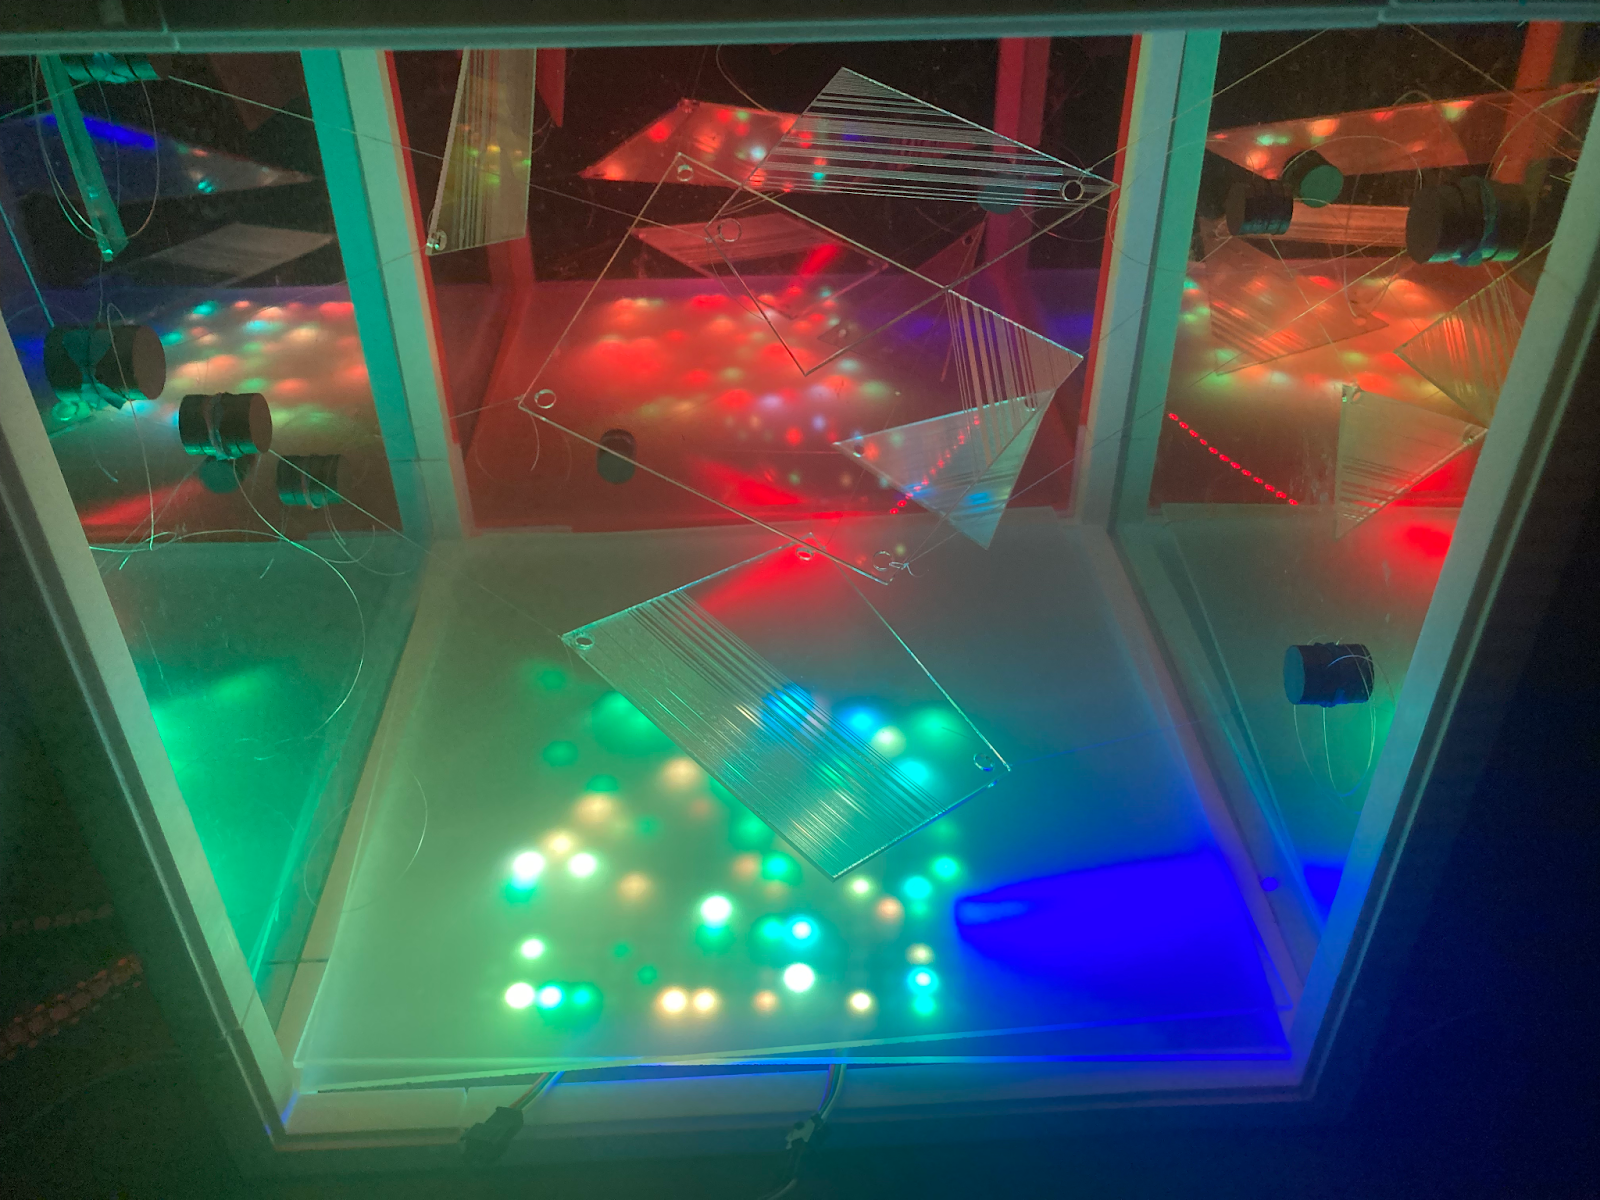
\includegraphics[width=\textwidth]{images/unnamed16.png}
  \end{minipage}
  \hfill
  \begin{minipage}[b]{0.4\textwidth}
    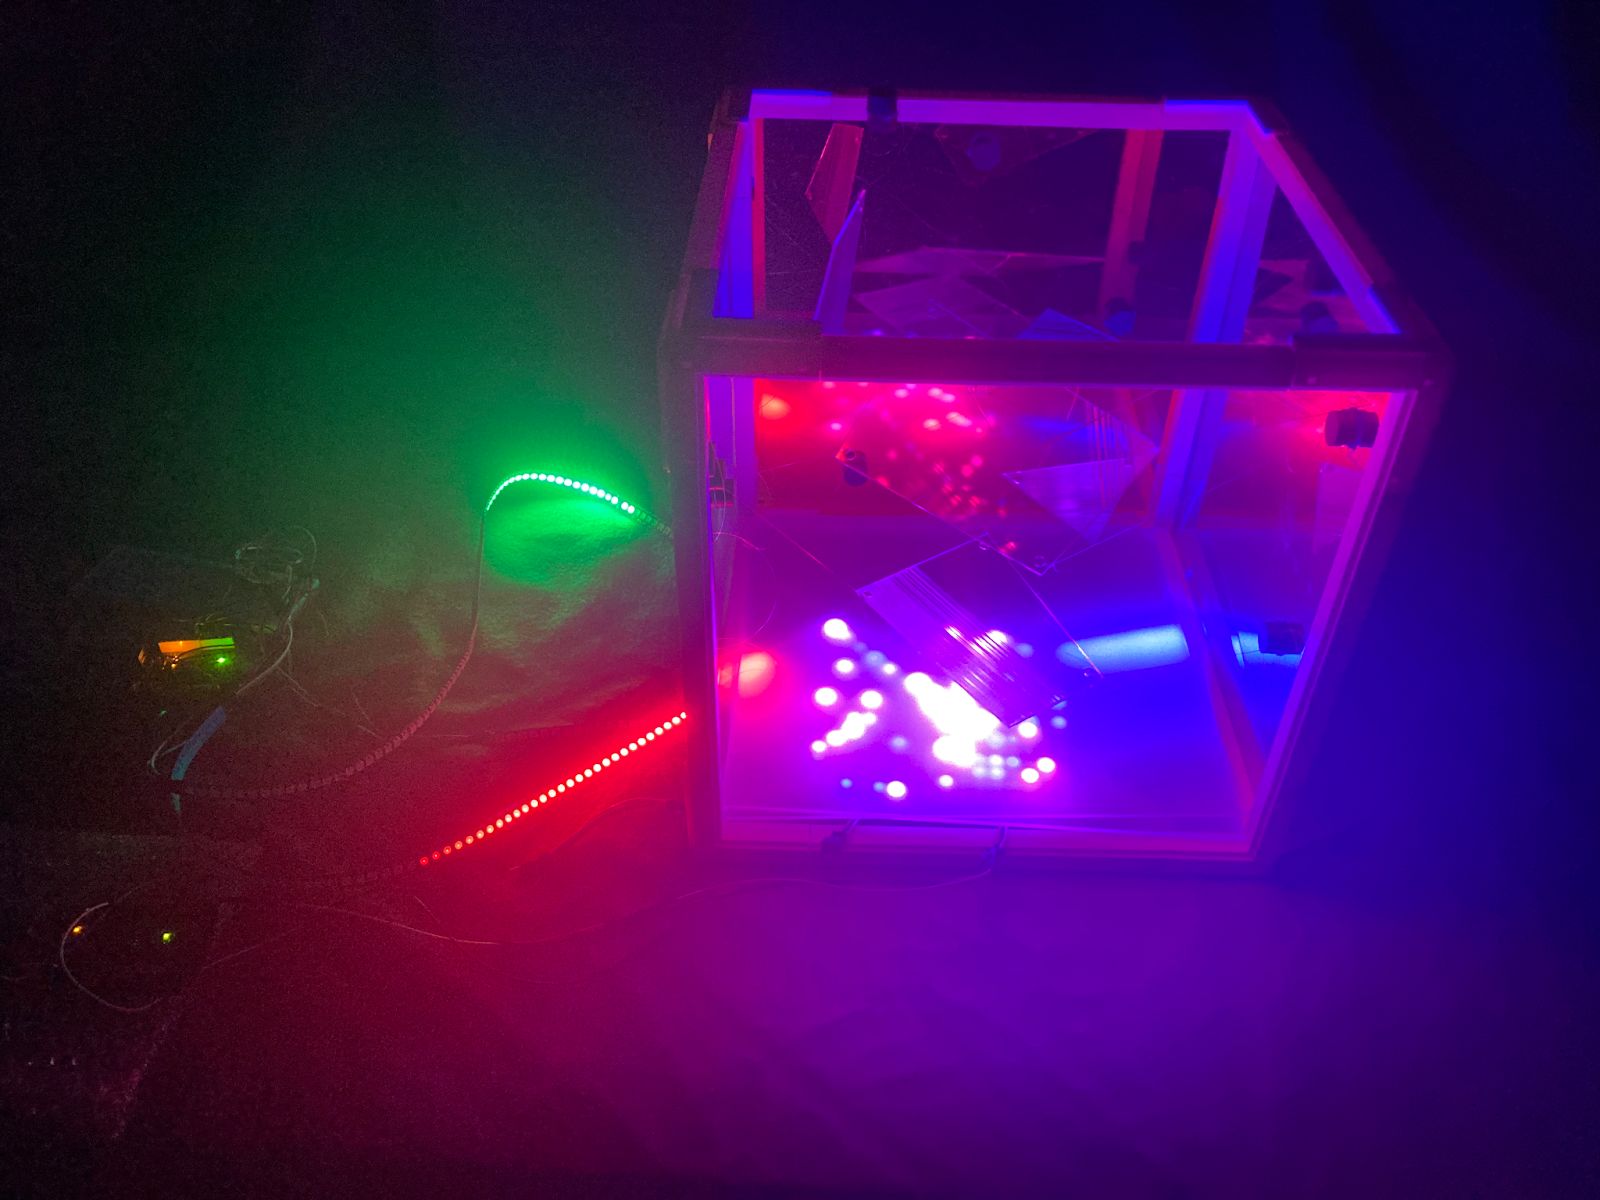
\includegraphics[width=\textwidth]{images/unnamed17.png}
  \end{minipage}
\end{figure}

\newpage

\section{Critique of Outcomes}
The most important and vital aspects of our design were the LED matrix display and the vibrant color variety. The LED matrix is important because it is one of the aspects of the prototype that most closely resembles one part of the phenomena of a cosmic ray. It is crucial for connecting the elegant displays with the educational aspect of the design. The vibrant color variety is vital because it is what initially grabs the attention of exhibit visitors. While presenting the design at the EUReCA research poster event, the bright colors on the LED matrix and strips are what initially brought many viewers toward our design, intrigued to learn more. 
We included the suspended glass panes to achieve the 2-dimensional focus of the prototype. We etched portions of the pieces to scatter the light produced by the LEDs throughout the reflections generated by the prototype’s walls. We do not think that these had the intended effect that we wanted. Or at least they didn’t achieve this goal to a satisfactory degree for our viewers. This may have a more impactful effect in a larger design where visitors can look up at the panes. In our small-scale prototype, viewers could only look directly at the panes from the side. Another option for modification, as per the reviewers, in a slightly larger version of the prototype, the pieces of plexiglass could be wider and expand closer to the walls of the design. There could also be a depth aspect added where only one piece is suspended per height level. This would probably require that the pieces of plexiglass be suspended more horizontally. An early concept sketch of the prototype included a grid ceiling from which the pieces of plexiglass would hang from. If this could be implemented practically, it may be worth including to some degree in later designs.
While interactivity is a key component of many exhibition displays, interactivity may not be necessary for all designs. While I believe that the interactivity was well implemented into our prototype, we rarely referred to it during presentations and reviewers did not tend to interact with the magnets suspending the plexiglass panes. Besides channeling an aspect of exhibition design, the interactivity of being able to move the suspended pieces of plexiglass did not contribute much to the overall impact of our design.

\newpage

\section{Next Steps}
\subsection{Technical}
A number of effects were individually investigated, These include: fading (light, sound), blur (of LED light, sound), randomization (particle paths, color), synchronization between different effects (such as different LED pattern displays. These effects should be coordinated together.

Randomization is important. For example, the directions for collisions of Protons with atoms could be random. 

There should be synchronization of LED strips and Matrix and sound and scintillator. The Scintillator detects muons and sends a trigger pulse after detection. This should be used to control various relevant LED displays.

More thought is required to coordinate the light with the structural elements - such as planes - of the exhibition. This requires controlling the interaction of colored light with various planes, such as frosted planes (blurring), mirrors, and diffraction gratings (e.g. the reflective surfaces of CDs).

It is important to coordinate colors (color theory) and map the colors to physics: The basics of color theory should be understood and considered when designing the exhibition (more on this later). This requires the ability to control the colors and intensities of different LEDs at the same time. 

There is a need to more fully understand the C++ code comprising the FastLED library - a comprehensive study of the relevant C++ code base is necessary. Time and effort was required to implement the FastLED functions. It would be useful and more efficient to have FastLED library documentation.

Augmented Reality could be used to display particle collisions superimposed on the geometry of the room. The exhibit could be made interactive via use of haptic controls.

Auxiliary exhibits might be interesting. For example, there could be side panels with interesting synapses of related physics (relativity, cosmic rays). Viewers would be interested in seeing an actual cloud chamber and its connection to the .

\subsection{Aesthetics}
A number of effects were individually investigated., in the context of aesthetics. These include: fading (light, sound), blur (of LED light, sound), randomization (particle paths, color), synchronization between different effects (such as different LED pattern displays. These effects should be coordinated as it relates to the effect of sensory input (e.g., light, sound) on the viewer. The design initially mimicked the collision of Protons with atmospheric atoms. However, nothing was left to the imagination; the display was too literal and not aesthetically pleasing.

A number of effects were therefore individually investigated in order to achieve a more aesthetically pleasing effect, These include: sequencing, fading (light, sound), blur (of LED light, sound), randomization (incoming and outgoing particle paths, color), synchronization between different effects (such as different LED displays.

Different LED displays were sequenced in order to tell a story. The LED strips and matrix displays need to be synchronized to each other and to the output of the scintillator. The LED strips and Matrix can also be synchronized to sound.

Randomization should be incorporated into all aspects of the design. For example, it could be applied to generate random directions for collision of Protons with atoms.

The effects of fading were investigated. For example, the LED string initially displayed a ‘moving’ white LED light. In later versions, different colored lights with a ‘fade’ control were used. This created a more aesthetically pleasing illusion of movement. The target atom could be composed of twinkling multi-colored LEDs (e.g., red and purple). The fading effect could also be applied to sound. 

More thought is required to coordinate the light with the structural elements - such as planes - of the exhibition. For example, a frosted plexiglass panel placed about 1 cm above the LEDs was used to blur the LED lights. The effect was very pleasing. Furthermore, actual diffraction gratings could be used to accentuate the interaction between light and the 2D planes. 

Coordinating colors (color theory): The basics of color theory should be understood and considered when designing the exhibition. For example, red next to green lights is jarring and not pleasing. The colors should also be mapped to the physics to tell a story. For example, hotter colors could represent higher energies. 

\subsection{Scalability} 
Scaling the cubic foot display to room-size dimensions involves consideration of many components. Thousands of LEDs might be desired. This, in turn increases the complexity of the circuit design as well as the complexity of the code. It further increases the cost of the hardware. 

The placement of lights needs reconsideration as well. Should the lights be placed above the viewers? Will the viewers be at the correct angle to see reflections of light from the planar surfaces? What about a 3D room sized LED array - mimicking the effect of a Stellarium?

Should sound be incorporated into the design? If so, how? Speakers or headphones could be used. Should there be background music? If so, what kind? One possibility is the The Planets Orchestral suite by Gustav Holst (\url{https://en.wikipedia.org/wiki/The_Planets}). Should there be interactive control of the sound? Should there be fading control by viewers?

The issue of safety should be considered. The current design of the planes contain sharp edges. This could be a problem if they are suspended above the viewers. 

\subsection{Financial}
Budget: the budget depends on many variables including labor costs (setting up the room-sized exhibit, labor, personnel, driver - if mobile), equipment (lighting (LED or other), Arduino boards, wiring). 

\subsection{Feasibility}
A feasibility study should first be conducted to determine the possible, realistic options. There are numerous constraints to consider: budget, time, manpower, technical know-how and knowledge database, whether the display is stationary vs. mobile, the power supply to name a few examples. 



\section{Conclusion}
Artistic and architectural design principles were used to create a sense of awe and scientific curiosity by illustrating the journey of a cosmic ray through the atmosphere by the interaction of patterned light with planar surfaces. To this end, a preliminary (cubic foot) design for an interactive, room-sized museum exhibition was created. Muons arriving on the Earth's surface are created indirectly as decay products of collisions of cosmic rays with particles of the Earth's atmosphere. The Muons are detected by a scintillator which sends a trigger pulse to an Arduino microcontroller, which in turn controls arrays of LEDs. The Arduino is programmed to create various patterns of light which then interact with the planar surfaces. The patterns artistically model the creation of Muons. Audience members join in the experience by controlling the positioning of the planar surfaces using magnets. Thus, the sense of awe and curiosity is instilled through visual representation of cosmic rays, inspiring participants to learn more about scientific discovery.

Participants should further extend the preliminary ideas presented here. Work needs to be carried out on how to scale-up the exhibition. A feasibility study should first be conducted and a budget determined. More comprehensive coordination between design elements such as 2D planes and various LED displays should be undertaken. The entire display should be triggered by a pulse from the Scintillator. Augmented Reality could be used to display simulated particle collisions superimposed on a display of the room. Viewer participation could be further extended via use of Haptic gloves so that viewers can control the placement of the 2D planes. Auxiliary exhibits might be interesting. For example, there could be side panels with interesting synopsis of related physics (historical discoveries, relativity, cosmic rays). Viewers would also be interested in seeing an actual cloud chamber and its connection to the artistic representation.


\end{document}
